\chapter{VQ H.264}
\label{chapter:chap5}

\section{Εισαγωγή}
\label{section:sect51}

\indent Στο τελευταίο κομμάτι αυτής της διπλωματικής έγινε η ενσωμάτωση του VQ (Vector Quantization) στον H.264 έτσι ώστε να μπορούμε να κάνουμε encoding και decoding με βάση τα VQ codebooks. Το να αντικατασταθεί όλος ο μηχανισμός κβαντοποίησης-μετασχηματισμού του encoder H.264 και ο αντίστοιχος μετασχηματισμός αντίστροφου μετασχηματισμού, κβαντοποίησης του decoder αποδείχθηκε αρκετά περίπλοκο και η ιδέα εγκαταλείφθηκε γρήγορα. Αντί για αυτό επιλέχθηκε να γίνει μια άλλη τροποποίηση η οποία αφήνει τον H.264 να κάνει όλες τις λειτουργίες του αλλά κάπου στο ενδιάμεσο γίνεται παρέμβαση  για να τροποποιηθούν τα residuals με το VQ.

\section{Encoding}
\label{section:sect52}

\indent Αφού πραγματοποιηθεί το Prediction o H.264 συνεχίζει με μετασχηματισμό και κβαντοποίηση των residuals. Έπειτα κάνει αντίστροφο μετασχηματισμό και αντίστροφη κβαντοποίηση (την διαδικασία που κάνει ο decoder) για να μπορεί να ανακατασκευάσει τα pixels με το σφάλμα που εισήχθηκε από την κβαντοποίηση. Αυτό είναι αναγκαίο διότι ο decoder γνωρίζει μόνο τα κβαντοποιημένα residuals αρά στον encoder θα πρέπει να παίρνουμε αποφάσεις μόνο με τα κβαντοποιημένα residuals. Με τον όρο αποφάσεις εννοείται ότι η επιλογή του καλύτερου Motion Vector στον encoder θα γίνει με βάσει τα ανακατασκευασμένα pixel. Επομένως κάπου στον encoder υπάρχει ένα σημείο που ανακατασκευάζει τα pixels, το οποίο βρίσκεται στο Σχήμα~\ref{fig:h264} στο σημείο μεταξύ Scaling \& Inv. Transform και Deblocking Filter. Επίσης αυτό το Σχήμα φανερώνει ότι τα reconstructed residuals χρησιμοποιούνται για να γίνεται το Motion Estimation.

\indent Η συνάρτηση που ο encoder Η.264 κάνει την πράξη $ Pixel_{reconstructed_i} = Residual_{reconstructed_i} + Pixel_{reference_i} $ βρίσκεται στο αρχείο blk\_prediction.c και ονομάζεται sample\_reconstruction. Δέχεται σαν ορίσματα έναν pointer στην ανακατασκευασμένη εικόνα, το μέγεθος του block καθώς και την θέση του στην εικόνα, τα Reference Pixels και τα Reconstructed Residuals.

\indent Η τακτική που ακολουθήθηκε ήταν να κωδικοποιηθεί το βίντεο με $QP=0$ (σχεδόν καθόλου απώλεια λόγω βαθμωτής κβαντοποίηση) άρα τα $Reconstructed Residuals = Original Residuals$. Αρά στην ουσία επιτεύχθηκε ο στόχος της αφαίρεσης του μηχανισμού μετασχηματισμού-κβαντοποίησης. Μετά από αυτό το βήμα, τροποποιήθηκε η συνάρτηση sample\_reconstruction έτσι ώστε προτού την πράξη ανακατασκευής των pixels να εισάγονται τα residuals του VQ. Αυτό επιτεύχθηκε πολύ απλά με τον Αλγόριθμο~\ref{alg:quantmb} όπου για την αναζήτηση του minimum distance χρησιμοποιήθηκε και εδώ ο αλγόριθμος FastNN για να επιταχύνει την διαδικασία του encoding. Μετά από αυτό το βήμα το καρέ ανακατασκευάζεται με βάση τα $VQ_{residuals}$, επομένως όλες οι αποφάσεις παίρνονται με βάση αυτά.

\indent Το επόμενο που έγινε είναι να αποθηκεύονται τα τελικά $VQ_{indices}$ σε ένα αρχείο. Όπως αναφέρθηκε για κάθε macroblock ο H.264 encoder δοκιμάζει όλα τα επιτρεπόμενα modes μέχρι να βρεθεί το καλύτερο, αυτό σημαίνει πως η συνάρτηση sample\_reconstruction θα κλιθεί όσες φόρες είναι και το πλήθος των επιτρεπόμενων modes ανά block. Επομένως χρειάζεται να κρατώνται τα προσωρινά $VQ_{indices}$ που γράφει o Αλγόριθμος~\ref{alg:quantmb} και κάθε φόρα που βρίσκεται ότι ένα mode είναι καλύτερο από το προηγούμενο να αντιγράφονται σε ένα global πίνακα που κρατάει τα καλύτερα VQ indices για κάθε macroblock.

\indent Αφού τελειώσει η διαδικασία αυτή για κάθε macroblock  τα $VQ_{indices}$ γράφονται σε ένα αρχείο. Στην παρούσα διπλωματική, τα $VQ_{indices}$ που γράφονται για κάθε Υ macroblock είναι $\frac{16*16}{4*4}=16$ όπου 16*16 η διάσταση του macroblock και $4*4=16$ η διάσταση του codebook. Επομένως γράφονται $2*16 = 32bytes$ ανά macroblock για το Υ και $2*8$ για το UV, το 2 bytes προκύπτει επειδή τα $VQ_{indices}\in[0,65535]$. Οι αλλαγές φαίνονται στο Σχήμα~\ref{fig:vqencoder}.

\begin{algorithm}[H]
\begin{algorithmic}[1]
\Function{quantize\_mb}{residuals,width,height,x,y,plane,mode}
\State{Load codebook for mode(Intra,Inter) and plane(Y,UV);}
\ForAll{subblocks with dimension dxd in block[x,y]}
    \State{$vq_i = $ codebook index with minimum distance from subblock;}
    \State{Replace dxd residuals with codebook[$vq_i$] data;}
    \State{Store $vq_i$ for subblock;}
\EndFor
\EndFunction
\end{algorithmic}
\caption{VQ Algorithm}
\label{alg:quantmb}
\end{algorithm}

\begin{figure}[H]
  \centering
  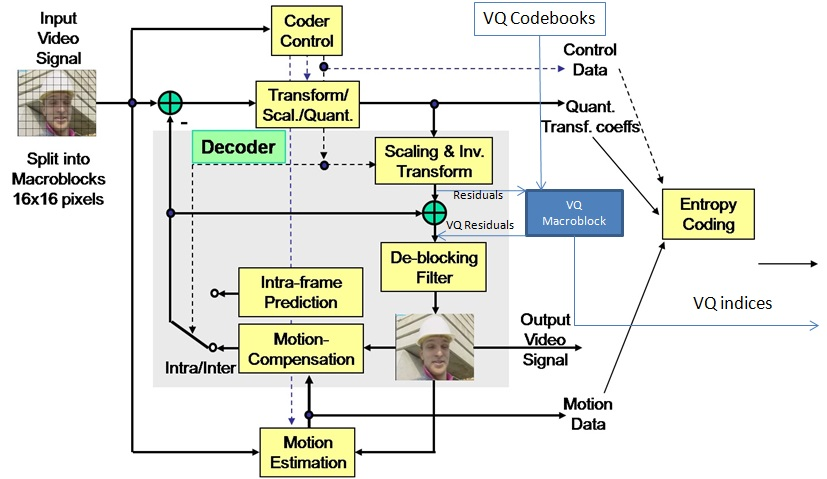
\includegraphics[width=0.7\textwidth]{chapter5/vqencoder.jpg}
  \caption{VQ H.264 Encoder Structure}
  \label{fig:vqencoder}
\end{figure}


\indent Για να παραμετροποιείται o JM Η.264 encoder προστέθηκαν οι παρακάτω επιλογές στο configuration file.

\begin{itemize}
    \item VQcodebook[YI,YB,YP,UVI,UVB,UVP] οπού δίνονται τα ονόματα των αρχείων των codebooks.
    \item VQindices οπού δίνεται το αρχείο των $VQ_{indices}$.
    \item VQdim οπου δίνεται η διάσταση $d$ των codebooks. Αν είναι 0 το VQ απενεργοποιείται.
    \item VQcblen οπού δίνεται το μήκος των codebooks $k$.
    \item Για να γίνει VQ πρέπει όλα τα QP να είναι 0.
\end{itemize}

\indent Ο VQ H.264 παράγει και ένα αρχείο ίδιο με αυτό του JM H.264 με κατάληξη .264 που περιέχει κατά κύριο λόγο τα Motion Vectors και κάποια headers. Επίσης εμπεριέχονται και τα συμπιεσμένα residuals, όμως  αυτά είναι άχρηστα για τον decoder αφού διαβάζονται από τα $VQ_{indices}$.

\section{Decoding}
\label{section:sect53}

\indent Στον decoder όπως είναι αναμενόμενο τα πράγματα είναι πιο απλά. Αφού επιτραπεί στον decoder να κάνει την διαδικασία αντίστροφης κβαντοποίησης και μετασχηματισμού, στο ίδιο ακριβώς σημείο με τον encoder παρεμβάλλεται ο Αλγόριθμος~\ref{alg:iquantmb}. Η συνάρτηση αυτή αντιστοιχίζει 16 $VQ_{indices}$ που διαβάζει από το αρχείο για κάθε ένα από τα 16 subblocks του macroblock με 16 $VQ_{vectors}$ για τα Y macroblocks,ακόμα 4 για το 8x8 macroblock του U και αντιστοίχος για το V κατά τον Αλγόριθμο~\ref{alg:iquantmb}. Τελικά ο decoder παίρνει την κύρια πληροφορία που είναι τα residuals από τα $VQ_{indices}$ ενώ τα headers, motion vectors από το αρχείο .264. Οι αλλαγές φαίνονται στο Σχήμα~\ref{fig:vqdecoder}.


\begin{figure}[H]
  \centering
  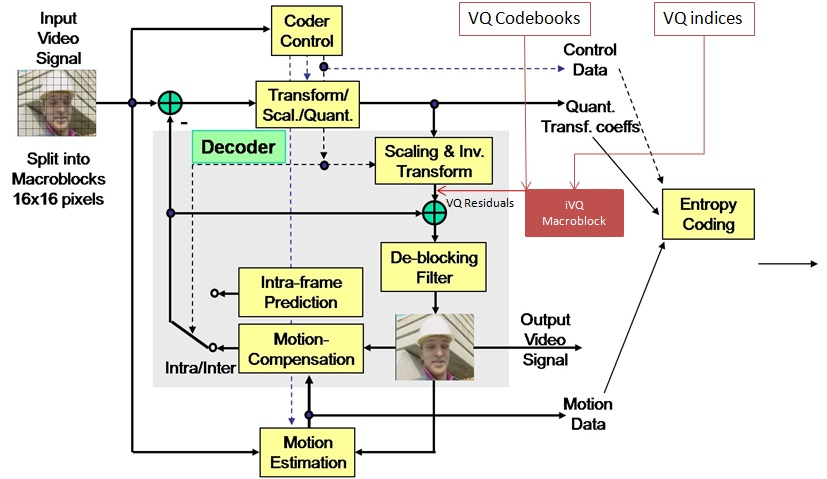
\includegraphics[width=0.7\textwidth]{chapter5/vqdecoder.jpg}
  \caption{VQ H.264 Decoder Structure}
  \label{fig:vqdecoder}
\end{figure}

\begin{algorithm}[H]
\begin{algorithmic}[1]
\Function{quantize\_mb}{residuals,width,height,x,y,plane,mode}
\State{Load codebook for mode(Intra,Inter) and plane(Y,UV);}
\ForAll{subblocks with dimension dxd in block[x,y]}
    \State{$vq_i = $ read $VQ_{index}$ from file for this position[x,y];}
    \State{Replace dxd residuals with codebook[$vq_i$] data;}
\EndFor
\EndFunction
\end{algorithmic}
\caption{Inverse VQ Algorithm}
\label{alg:iquantmb}
\end{algorithm}

\indent Για να παραμετροποιείται o JM Η.264 decoder προστέθηκαν οι παρακάτω επιλογές στο configuration file.

\begin{itemize}
    \item VQcodebook[YI,YB,YP,UVI,UVB,UVP] οπού δίνονται τα ονόματα των αρχείων των codebooks.
    \item VQindices οπού δίνεται το αρχείο των $VQ_{indices}$.
    \item VQdim οπου δίνεται η διάσταση $d$ των codebooks. Αν είναι 0 το VQ απενεργοποιείται.
    \item VQcblen οπού δίνεται το μήκος των codebooks $k$.
\end{itemize}